\documentclass[12pt, letterpaper]{article}
\usepackage[utf8]{inputenc}
\usepackage{graphicx}
\usepackage{indentfirst}
\usepackage{amsmath}
\usepackage{esint}
\usepackage{float}
\usepackage{amssymb}
\usepackage{siunitx}
\usepackage{physics}
\usepackage{hyperref}
\hypersetup{
    colorlinks=true,
    linkcolor=black,  
    urlcolor=cyan,
    }
\graphicspath{ {images/} }

\title{Projeto 1 - F328}
\author{Rian Radeck Santos Costa - 187793 \\ Grupo I06}
\date{15 de Junho de 2022}
\renewcommand*\contentsname{Sumário}

\begin{document}

\maketitle
\newpage
\tableofcontents
\newpage

\section{Enunciado e avisos}
    O objetivo deste projeto é estudar a radiação emitida por uma partícula carregada e estudar o resultado em algumas situações reais. Todas as referências bibliográficas estão no fim desse documento.

    \begin{enumerate}
        \item \textbf{\textit{Radiação emitida:}} Para calcular a radiação emitida, considere uma carga que está inicialmente movendo-se em velocidade constante $v_0$ até $t = 0$. Ela sofre então uma aceleração negativa constante com valor $a = v_0/\tau$, a qual leva a partícula para o repouso em um tempo $t = \tau$. Vamos assumir que $v_0 \ll c_0$, onde $c_0$ é a velocidade da luz no vácuo (veja a figura).

        \begin{figure}[h]
            \centering
            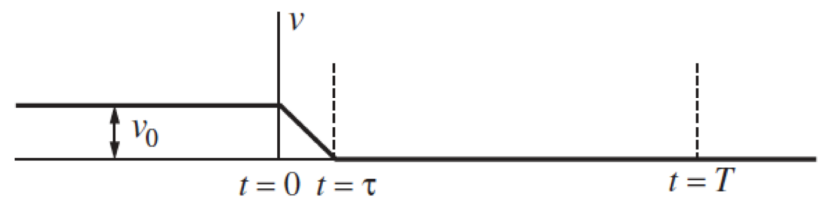
\includegraphics[width=0.8\textwidth]{start}
            \label{fig:fig0}
        \end{figure}

        Calcule a energia total do campo eletromagnético transversal (onda eletromagnética) e calcule a potência irradiada.

        \item \textbf{\textit{Átomo de hidrogênio:}} Considere um modelo tipo de Bohr para o átomo de hidrogênio, isto é, o elétron realizando uma órbita circular em torno do próton. Utilize valores realistas para o raio de Bohr do átomo de hidrogênio e estime o tempo que levaria para o elétron colapsar no núcleo.

        \item \textbf{\textit{Radiação síncrotron:}} Para resolver uma situação relativística, transforme o problema para um    referencial $F'$ no qual a partícula move-se lentamente. Nesse referencial você pode utilizar o resultado obtido anteriormente. Depois transforme para o referencial desejado. Considere agora um elétron altamente relativístico $(\gamma \gg 1)$ movendo-se perpendicularmente a um campo magnético $B$. Ele é continuamente acelerado perpendicularmente ao campo e deve irradiar. Calcule a radiação síncrotron, isto é a potência emitida pelo elétron. Sugestão: 

    \begin{enumerate}
        \item Qual a relação entre a potência irradiada, $P_{rad}$ emitida em um referencial $F$ e a potência irradiada, $P_{rad}'$ em um referencial $F'$ que é um referencial inercial em relação a $F$?
        \item Transforme o problema para um referencial $F'$ que esteja momentaneamente movendo-se com a partícula. Transforme (relativisticamente) os campos e encontre $P_{rad}'$. Faça a transformação da potência irradiada de volta para o referencial do laboratório. De posse do resultado, comente as implicações do seu resultado para um colisor circular (tipo LHC) e um síncrotron (tipo Sirius).
    \end{enumerate}
    \end{enumerate}

\newpage
\section{Radiação emitida}
    \par
    A primeira observação que devemos fazer é que enquanto uma partícula carregada está em movimento ela tem um campo fácil de ser observado, como na figura 1.
    
    \begin{figure}[h]
        \centering
        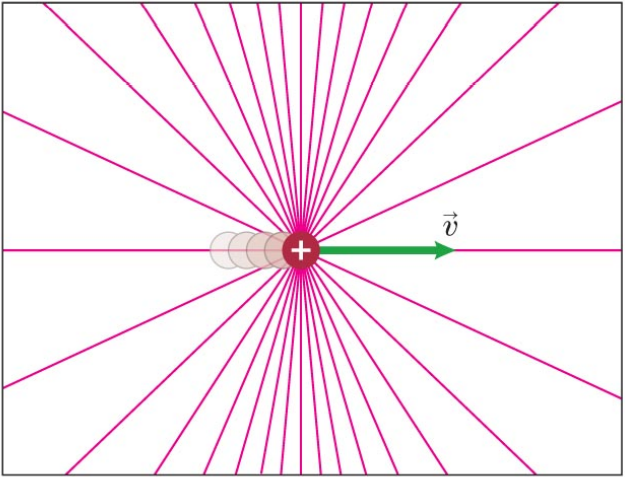
\includegraphics[width=0.4\textwidth]{moving particle}
        \\{Figura 1: Linhas de campo de uma carga com velocidade constante}
        \label{fig:fig1}
    \end{figure}

    Sabemos que a informação sobre a nossa partícula para qualquer ponto no espaço se move na velocidade da luz, portanto o nosso pulso se move nessa velocidade. Também sabemos que, de acordo com as leis do eletromagnetismo clássico, toda partícula que sofre uma aceleração emite radiação e faz um pulso eletromagnetico no período de aceleração, dividindo o espaço em três regiões, a interna, que já notou que a partícula está se movendo, a externa, que ainda não notou isso e a intermediária, que chamamos de \textit{ring of kinks}.

    \begin{figure}[h]
        \centering
        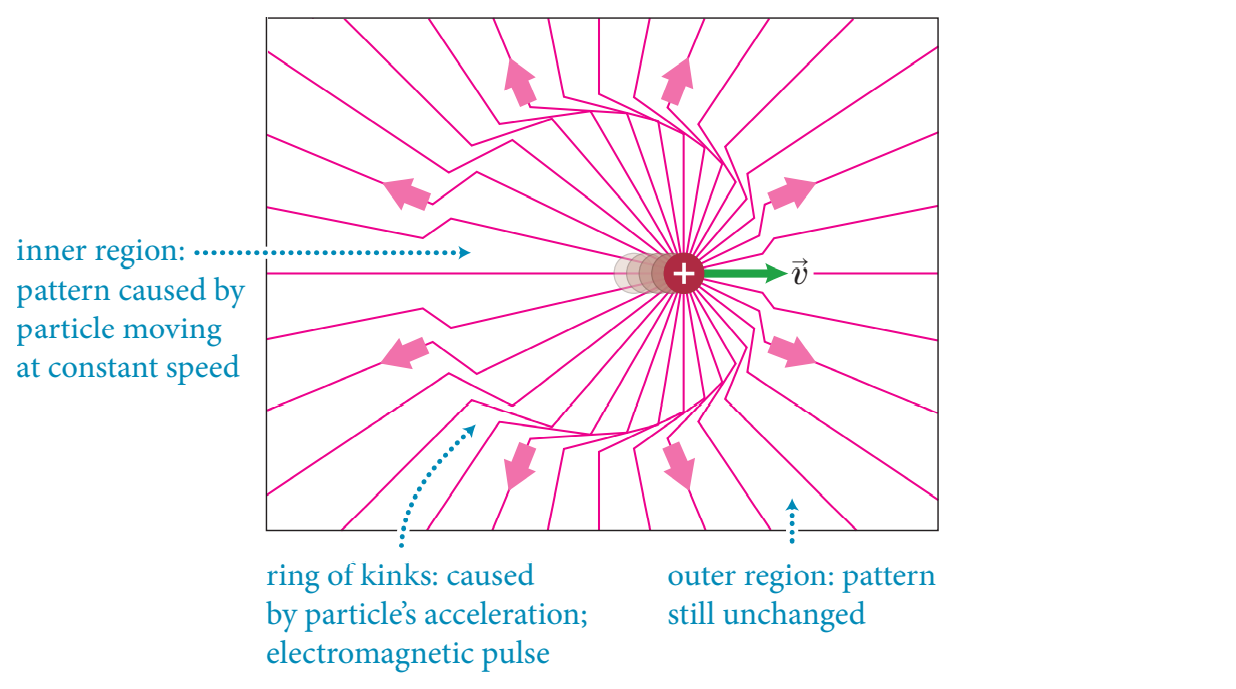
\includegraphics[width=0.7\textwidth]{pulse}
        \\{Figura 2: Partícula carregada que saiu do repouso e mantém velocidade constante}
        \label{fig:fig2}
    \end{figure}

    Vamos então marcar alguns pontos importantes para calcularmos o campo na região intermediária e a potência irradiada. Tome um tempo $t = T \gg \tau$, teremos o seguinte diagrama:

    \begin{figure}[h]
        \centering
        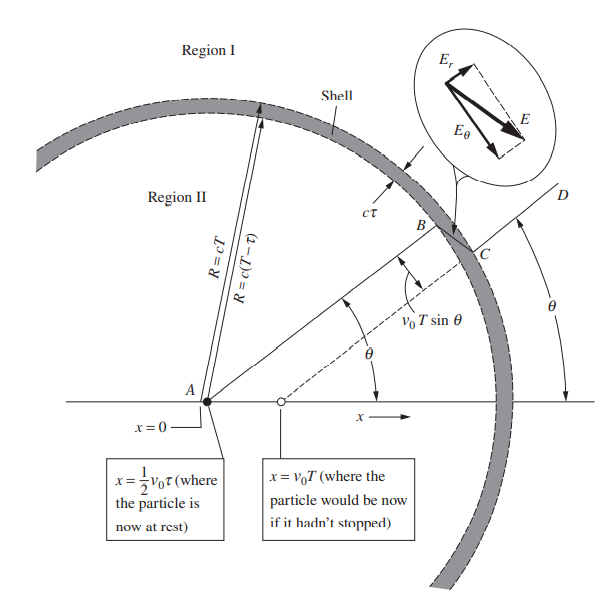
\includegraphics[width=0.7\textwidth]{diagrama}
        \\{Figura 3: Diagrama para um instante $t = T \gg \tau$, um longo tempo após a parada da partícula}
        \label{fig:fig3}
    \end{figure}

    Vamos definir $x = 0$ como o lugar no espaço onde a nossa partícula começou a ser desacelerada e $t = 0$ como o momento que ela começou a ser desacelerada. Definindo esses referenciais, conseguimos definir nossas regiões e a posição onde nossa partícula irá parar, que será definida pela equação de Torricelli $v^2 = v_0 ^2 + 2a\Delta S$. Portanto nossa partícula estará no repouso em $x = \frac{1}{2} v_0 \tau$, já que $a = v_0 /\tau$. Outra posição importante para o nosso diagrama é $x = v_0 T$, que é onde a partícula estaria se nunca tivesse sido desacelerada. Esse ponto é importante pois é onde os pontos no espaço após o pulso eletromagnético pensam que nossa partícula está, já que eles nunca receberam a informação da desaceleração.

    Vamos então definir nossas regiões. Aqui, ``Region I" é a região externa ao pulso, que ainda não recebeu a informação que a partícula parou, ou seja está a uma distância maior que $cT$ do ponto $x = 0$ $(R > cT)$. Similarmente, ``Region II'' é a região que já recebeu essa informação, portanto sua distância ao ponto $x = 0$ é $R \leq c(T - \tau)$ e a região do pulso que está definida no diagrama como ``Shell'' é a que está entre as duas definidas anteriormente e tem espessura de $c\tau$.

    Agora devemos nos perguntar: Qual o formato de uma linha de campo na região de transição? Devemos olhar para a lei de Gauss para obter a resposta. Tome uma linha de campo que sai do ponto A (partícula parada) e atinge o ponto B, no início da região de transição. Essa linha faz uma angulação $\theta$ com o eixo de viagem da partícula. Sabemos então que esse cone de angulação possui uma certa quantidade de fluxo o atravessando (veja o cone vermelho na imagem.) Se tomarmos um cone que é definido por CD e o eixo de viagem da partícula, de mesmo tamanho porém com seu centro em $x = v_0T$ (veja o cone azul na imagem), ele terá o mesmo $\theta$ e, portanto, terá a mesma quantidade de fluxo atravessando-o. (Observe que isso só é verdade pois $v_0$ é pequeno quando comparado a $c$, o que nos deixa ignorar efeitos relativísticos.) Aliando isso com o fato de linhas de campo não se cruzarem podemos concluir que as linhas de campo AB e CD são a mesma linha e devem estar conectadas por BC.

    \begin{figure}[H]
        \centering
        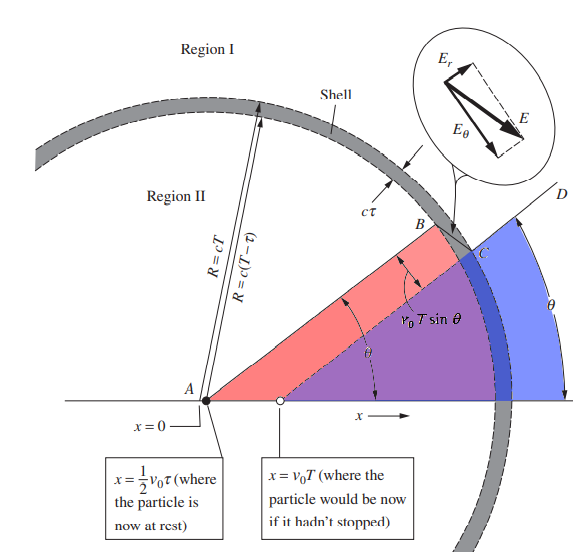
\includegraphics[width=0.65\textwidth]{highlight}
        \\{Figura 4: Cones de fluxo destacados do diagrama.}
        \label{fig:fig4}
    \end{figure}

    Vamos finalmente calcular o valor do campo na região intermediária. Como sabemos a direção do campo, devemos calcular suas componentes $E_r$ (componente radial) e $E_\theta$ (componente transversal). Da geometria do problema podemos concluir que:
    
    \begin{equation} \label{eq1}
    \frac{E_\theta}{E_r} = \frac{v_0 T\sin{\theta}}{c\tau}
    \end{equation}

    Observe que $E_r$ não muda na região intermediária, para ver isso basta tomar uma gaussiana com $c(t - \tau) < R \leq cT$, veremos que o campo $E_r$ é constante e a carga envolvida é a mesma. Se tomarmos uma gaussiana equivalente a parte externa da casca $(R = cT)$ podemos calcular $E_r$.

    \begin{equation} \label{eq2}
    \begin{split}
        \oiint E_r \delta \vec{A} &= \frac{q_{env}}{\epsilon_0} \\
        E_r(4\pi R^2) &= \frac{q}{\epsilon_0} \\
        E_r &= \frac{q}{4\pi\epsilon_0R^2} \\
        E_r &= \frac{q}{4\pi\epsilon_0c^2T^2} 
    \end{split}
    \end{equation}

    Utilizando o resultado obtido, substituimos na equação \ref{eq1}:

    \begin{equation} \label{eq3}
        E_\theta = \frac{v_0T\sin{\theta}}{c\tau}E_r = \frac{qv_0\sin{\theta}}{4\pi\epsilon_0c^3T\tau}
    \end{equation}

    mas, $v_0 / \tau = a$ e $cT = R$, então nosso resultado é melhor representado por:

    \begin{equation} \label{eq4}
        E_\theta = \frac{qa\sin{\theta}}{4\pi\epsilon_0c^2R}
    \end{equation}

    Como podemos concluir, $E_\theta$ é proporcional a $1/R$ e, com o passar do tempo, $E_r$ se torna negligível quando comparado a $E_\theta$ portanto, $E$ será perpendicular a $\vec R$. De acordo com as equações de Maxwell um campo elétrico variável gera uma corrente de deslocamento, o que causa um campo magnético $B$ perpendicular a $E$ e a $\vec R$, isso é uma das propriedades fundamentais de uma onda eletromagnética.

    Vamos então calcular a energia que está guardada no campo elétrico transversal para toda a região intermediária. A densidade de energia de um campo elétrico $E$ em determinada região do espaço é definida pela equação $\frac{1}{2}\epsilon_0E^2$, assim para nosso campo elétrico transversal nossa densidade de energia será:

    \begin{equation} \label{eq5}
        \frac{\epsilon_0E_\theta^2}{2} = \frac{q^2a^2\sin^2{\theta}}{32\pi^2\epsilon_0R^2c^4}
    \end{equation}    

    Como o volume da casca será $4\pi R^2 c\tau$ e o valor médio de $\sin^2{\theta}$ sobre uma esfera completa é $2/3$ já que $x^2 + y^2 + z^2 = R^2 \Rightarrow \overline{x^2} = R^2/3$ e $\cos^2{\theta} = x^2/R^2$, chegamos ao resultado que $\overline{\cos^2{\theta}} = \overline{x^2} /R^2 = 1/3 \Rightarrow \overline{\sin^2{\theta}} = 2/3$. Podemos concluir que a energia total que atravessa o campo elétrico é:

    \begin{equation} \label{eq6}
        \frac{q^2a^2}{32\pi^2\epsilon_0R^2c^4}\frac{2}{3}4\pi R^2c\tau = \frac{q^2a^2\tau}{12\pi\epsilon_0c^3}
    \end{equation}    

    Para sabermos quanta energia nossa onda magnética carrega vamos olhar para as equações de Maxwell:

    \begin{equation}
    \begin{split}
        \curl\textbf{E} &= -\frac{1}{c}\frac{\delta\textbf{B}}{\delta t} \\
        \curl\textbf{B} &= \frac{1}{c}\frac{\delta\textbf{E}}{\delta t} + \frac{4\pi}{c}\textbf{J} \\
        \div\textbf{E} &= 4\pi\rho \\
        \div\textbf{B} &= 0
    \end{split}
    \end{equation}

    Perceba que em um espaço vazio, onde $\rho$ e $\textbf{J}$ são zero, as equações são traduzidas para o seguinte

    \begin{equation}
    \begin{split}
        \curl\textbf{E} &= -\frac{1}{c}\frac{\delta\textbf{B}}{\delta t} \\
        \curl\textbf{B} &= \frac{1}{c}\frac{\delta\textbf{E}}{\delta t} \\
        \div\textbf{E} &= 0 \\
        \div\textbf{B} &= 0
    \end{split}
    \end{equation}

    Assim fica claro que quando uma onda elétrica viaja pelo espaço vazio, uma onda magnética de mesma intensidade e perpendicular a ela (e a direção de propagação) deve surgir, como na figura a seguir

    \begin{figure}[h]
        \centering
        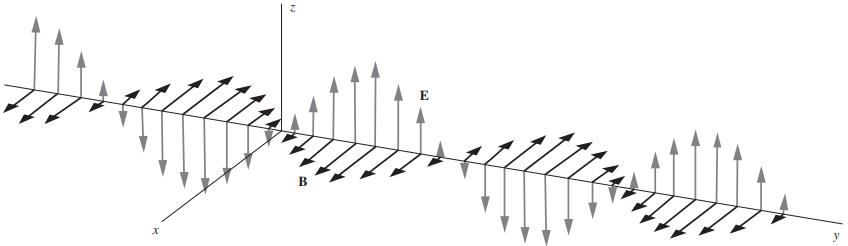
\includegraphics[width=0.9\textwidth]{wave}
        \\ Figura 5: Onda eletromagnética viajando pelo espaço vazio no eixo $y$
    \end{figure}

    Assim a energia total de nossa onda será o dobro da energia da onda elétrica.

    \begin{equation} \label{eq7}
        \textrm{Energia total propagada pelo campo eletromagnético} =\frac{q^2a^2\tau}{6\pi\epsilon_0c^3}
    \end{equation}

    Perceba que o raio $R$ não participa mais da nossa equação, isso significa que essa quantidade de energia simplesmente passeia pelo espaço, se distanciando da partícula, com a velocidade da luz, a partir do local da desaceleração $(x = 0)$. Como $\tau$ é o período da desaceleração, e também a duração do pulso eletromagnético, podemos declarar que a potência irradiada durante o processo de desaceleração foi:

    \begin{equation} \label{eqMaster}
        P_{rad} = \frac{q^2a^2}{6\pi\epsilon_0c^3} = \mu_0\frac{q^2a^2}{6\pi c}
    \end{equation}

    Esse resultado é bem conhecido e chamado de fórmula de Larmor.

    Perceba também que não importa se nossa partícula está acelerando ou desacelerando, só importa a magnitude da aceleração. Complementando a ideia de diferentes referenciais, $P_{rad}$ é uma grandeza invariante de \textit{Lorentz}, já que $P_{rad}$ é \textit{energia / tempo}, e energia se transforma como o tempo na teoria da relatividade especial de Einstein.

    Aqui nós obtemos o seguinte resultado: A equação \ref{eqMaster} nos dá a taxa instantânea de irradiação de energia de uma partícula carregada que sofre uma variação de aceleração. Isso é muito útil e pode ser utilizado em diversas aplicações, afinal, ondas eletromagnéticas movem o mundo.

\newpage
\section{Átomo de hidrogênio}

    Aqui vamos trabalhar com o modelo atómico de Rutherford e não o de Bohr, já que Bohr fez correções ao modelo planetário de Rutherford utilizando ideias de teoria quântica de Planck, os conceitos de Einstein sobre o fóton e a mecânica clássica Newtoniana. Recomendo a leitura da seção 42.3 do livro ``Física para cientistas e engenheiros, 2ª ed. (Brasil), 2018", dos autores Jewett \& Serway para uma decrição mais detalhada do modelo atómico de Bohr.

    \subsection{Um breve resumo sobre o átomo de hidrogênio de Bohr:}

    Bohr propôs que o elétron na órbita do átomo de hidrogênio, só ocupasse determinadas regiões do espaço, onde ele não irradiaria e perderia energia colapsando no núcleo. Essas órbitas propostas eram circulares e ele as chamou de ``estados estacionários".

    Bohr propôs que o elétron poderia ``saltar" de uma órbita (estado estacionário) para outra se liberasse energia em forma de fóton, indo para uma órbita menos energética, ou se recebesse a energia de um fóton, o que causaria que o elétron fosse para um estado mais energético.

    Uma análise um pouco mais quantitativa é dizer que as órbitas permitidas seriam aquelas que o momento angular do elétron seria um múltiplo inteiro de $\hslash = h/2\pi$, onde $h$ é a constante de Planck.

    \begin{figure}[h]
        \centering
        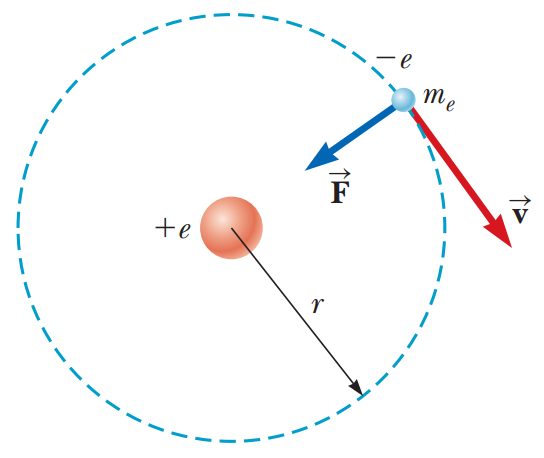
\includegraphics[width=0.5\textwidth]{bohr}
        \\{Figura 6: Modelo do átomo de hidrogênio de Bohr}
        \label{fig:bohr}
    \end{figure}

    \subsection{Tempo de colapso}

    % \newpage
    Bom, esclarecido o comportamento do átomo de Bohr, vamos então trabalhar com o modelo de Rutherford, que permite raios arbitrários para a órbita do elétron.

    De acordo com a teoria do eletromagnetismo de Maxwell, cargas com aceleração centrípeta com frequência de revolução $f$, devem irradiar ondas eletromagnéticas com frequência $f$, assim o modelo átomico de Rutherford é guiado para autodestruição.

    \begin{figure}[H]
        \centering
        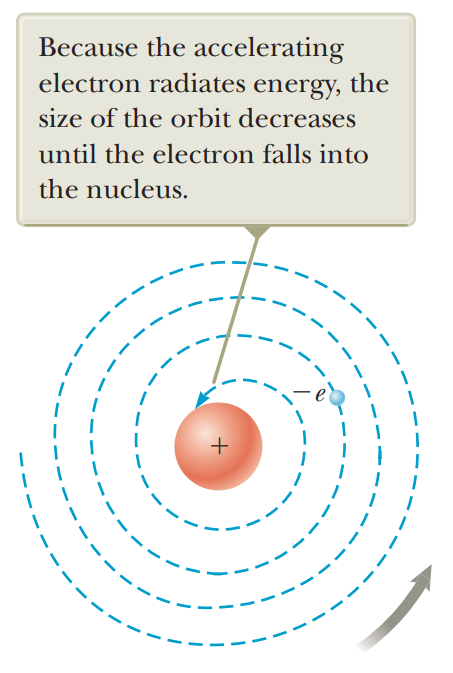
\includegraphics[width=0.5\textwidth]{ruth}
        \\{Figura 7: O modelo átomico de Rutherford prevê seu decaimento}
        \label{fig:ruth}
    \end{figure}

    Vamos esclarecer alguns parâmetros para o nosso problema:
    \begin{itemize}
        \item O elétron está sempre em uma órbita quase que perfeitamente circular ($v \approx v_\theta \gg v_r$).
        \item A taxa de perda energética é bem representada pelo resultado clássico obtido na seção 2 desse documento.
    \end{itemize}

    Dessa maneira podemos equacionar que a força centrípeta será igual a força elétrica.
    \begin{equation}
        \frac{mv^2}{R} = \frac{e^2}{4\pi\epsilon_0R^2} \Leftrightarrow \frac{v^2}{R} = \frac{e^2}{4\pi\epsilon_0mr^2}
    \end{equation}
    onde $v^2/R$ é a aceleração do elétron.

    Vamos agora equacionar a energia total presente no sistema:
    \begin{equation}
        E = K + U = \frac{mv^2}{2} - \frac{e^2}{4\pi\epsilon_0R} = -\frac{e^2}{8\pi\epsilon_0R}
    \end{equation}
    onde $E$ é a energia total do sistema, $K$ é a energia cinética e $U$ a energia potencial.

    O período de rotação será

    \begin{equation}
        T = \frac{2\pi R}{v} = \frac{1}{\abs{e}}\times4\sqrt{\pi^3\epsilon_0mR}
    \end{equation}

    Podemos supor que a energia irradiada em uma revolução é muito menor que a energia total, o que nos deixa trabalhar com $R$ sendo uma função do tempo, portanto $R = R(t)$. Então vamos calcular a energia irradiada em uma revolução:

    \begin{equation}
        P_{rad}T = \mu_0\frac{e^2a^2}{6\pi c}T = \mu_0\frac{e^2v^2}{6\pi cR^4}
    \end{equation}

    Vamos agora calcular a mudança na energia total em uma revolução:

    \begin{equation}
    \begin{split}
        E(R(t + T)) - E(R(t)) &= -\frac{e^2}{8\pi\epsilon_0R(t + T)} - [-\frac{e^2}{8\pi\epsilon_0R(t)}] \\
        &\approx \frac{e^2T}{8\pi\epsilon_0R^2(t)}\frac{\delta R(t)}{\delta t}
    \end{split}
    \end{equation}
    pois $R(t + T) = R(T) + T\frac{\delta R(t)}{\delta t}$. Tabém é comum escrever $\frac{\delta R(t)}{\delta t}$ como $\dot{R}(t)$

    Como podemos ver chegamos a uma equação diferencial

    %(igualando a potência irradiada com a mudança de energia)
    \begin{equation}
        \frac{\delta R(t)}{\delta t} = -\frac{\mu_0ce^4}{12\pi^2m^2R^2(t)} \Leftrightarrow R^2(t)\frac{\delta R(t)}{\delta t} = -\frac{\mu_0ce^4}{12\pi^2m^2}\delta t
    \end{equation}

    \newpage
    Integrando a equação 16:

    \begin{equation}
    \begin{split}
        \int R^2\delta R &= -\frac{\mu_0ce^4}{12\pi^2m^2} \int\delta t \\
        \frac{R^3}{3} &= -\frac{\mu_0ce^4}{12\pi^2m^2}t + K
    \end{split}
    \end{equation}

    onde $K$ é a constante de integração. Se tomarmos no tempo $t = 0$ nosso raio como o raio de Bohr $R_0$, nossa constante $K = \frac{R_0^3}{3}$ e temos um resultado mais representativo para a realidade que será:

    \begin{equation}
        R_0^3 - R^3(t) = \frac{\mu_0ce^4}{4\pi^2m^2}t
    \end{equation}

    Finalmente podemos obter o tempo de colapso do átomo de hidrogênio de Rutherford/Bohr

    \begin{equation}
        R(\tau) = 0 \Rightarrow \tau = \frac{4\pi^2m^2}{\mu_0^2ce^4}R_0^3
    \end{equation}

    Utilizando 
    $$c = \SI[inter-unit-product =\cdot]{2.99e8}{\meter\per\second}$$
    $$m = \SI{9.11e-31}{\kilogram}$$
    $$e = \SI{-1.6e-19}{\coulomb}$$
    $$\mu_0 = \SI[inter-unit-product =\cdot]{1.256e-6}{\kilogram\meter\per\second\squared\per\ampere\squared}$$
    $$R_0 = \SI{5.29e-11}{\meter}$$
    obtemos
    $$\tau = \SI{1.57e-11}{\second}$$


\newpage
\section{Radiação Síncrotron}

    Seja $v$ a velocidade do elétron no referencial $F$ na terra, vamos calcular então seu campo no referencial $F'$ que é o referencial que se move com o elétron em um dado instante $\delta t$. Usando as transformadas de Lorentz, o campo elétrico em $F'$ será $E' = \gamma v\times B'$.

    Vamos então calcular $E'$ e $B'$ de acordo com as trasnformadas de Lorentz
    \begin{equation}
    \begin{split}
        E' &= -v \times B \\
        B' &= \frac{1}{c^2}v \times E \\
        E'_x &= E_x \\
        E'_y &= \gamma(E_y - vB_z) \\
        E'_z &= \gamma(E_z + vB_y) \\
        B'_x &= B_x \\ 
        B'_y &= \gamma(B_y + \frac{v}{c^2}E_z) \\
        B'_z &= \gamma(B_z - \frac{v}{c^2}E_y) \\
    \end{split}
    \end{equation}
    perceba então que para nossa situação $B' = B$.

    Antes de prosseguir com os cálculos, observe que em $F'$
    $$
    \Delta t = \gamma\Delta t' \iff \Delta x' = 0
    $$$$
    U = \gamma U' \iff p' = 0
    $$

    Aqui $U$ representa a energia. Isso implica então que $\Delta U/\Delta t = \Delta U'/\Delta t' \Longrightarrow P = P'$ então, antes de qualquer cálculo, sabemos que nossa radiação emitida será a mesma nos dois referenciais. Vamos então calcular $P'$ em relação ao campo magnético $B$ e as constantes relativísticas.

    Como já descobrimos $E' = \gamma v\times B$, esse campo faz com que a partícula acelere no referencial $F'$, ou seja $v'$ começa a crescer e será diferente de 0 em $F'$ após o instante que estamos analisando. Desenvolvendo a equação $F = m_ea \Rightarrow eE' = m_ea \Rightarrow a = eE'/m_e$, obtemos a aceleração do elétron. Utilizando o resultado da equação \ref{eqMaster}, essa aceleração causa uma irradiação no elétron a uma taxa de
    \begin{equation} \label{eq13}
        P' = \frac{q^2a^2}{6\pi\epsilon_0c^3} = \frac{e^2(eE'/m_e)^2}{6\pi\epsilon_0c^3} = \frac{e^4\gamma^2v^2B^2}{6\pi\epsilon_0c^3m_e^2} \approx \frac{e^4\gamma^2B^2}{6\pi\epsilon_0m_e^2c}
    \end{equation}
    e a aproximação final foi feita devido ao fato de nosso elétron ser altamente relativístico.

    Veja que após o instante de tempo $\delta t$ devemos escolher um novo referencial $F''$ que o elétron esteja parado ($v'' = 0$), já que ele está em constante processo de aceleração ($v' \neq 0$ após um $\delta t$), um instante após o outro.

\newpage
\section{Referências}
    \subsection{Figuras}
    Figuras 1 e 2: Mazur, Eric, Principles \& Practice of Physics, Pearson Education (2015)

    Figuras 3 e 5: Purcell, Edward M. \& Morin, David J., Electricity and Magnetism, Cambridge University Press (3rd edition, 2013) (1st edition, vol. 2 da Coleção de Física de Berkeley, 1963).

    Figuras 6 e 7: Jewett \& Serway, Física para cientistas e engenheiros, Cengage (9a ed. (EUA), 2a ed (Brasil), 2018).

    \subsection{Referências bibliográficas}
    Mazur, Eric, Principles \& Practice of Physics, Pearson Education (2015)

    Bauer, Westfall \& Dias, Física para Universitários, McGraw-Hill  (1a ed., 2012)

    Halliday, Resnick \& Walker, Fundamentos de Física, LTC (10a ed., 2012).

    Jewett \& Serway, Física para cientistas e engenheiros, Cengage (9a ed. (EUA), 2a ed (Brasil), 2018).

    Purcell, Edward M. \& Morin, David J., Electricity and Magnetism, Cambridge University Press (3rd edition, 2013) (1st edition, vol. 2 da Coleção de Física de Berkeley, 1963).

    Nussenzveig, H.M., Eletromagnetismo, Curso de Física Básica, vol. 3, Ed. Edgard Blücher, (1997).


    \href{https://en.wikipedia.org/wiki/Abraham\%E2\%80\%93Lorentz_force}{Abraham–Lorentz force (Wikipedia)}

    \href{https://en.wikipedia.org/wiki/Larmor_formula}{Larmor formula (Wikipedia)}

    \href{https://en.wikipedia.org/wiki/Bohr_radius}{Bohr radius (Wikipedia)}

    \href{https://en.wikipedia.org/wiki/Vacuum_permeability}{Vacuum permeability (Wikipedia)}    

    \href{http://physicspages.com/pdf/Electrodynamics/Li%C3%A9nard%27s%20generalization%20of%20the%20Larmor%20formula%20for%20an%20accelerating%20charge.pdf}{LIÉNARD’S GENERALIZATION OF THE LARMOR FORMULA FOR AN ACCELERATING CHARGE (physicspages)}

    \href{https://physicspages.com/pdf/Electrodynamics/Synchrotron%20radiation.pdf}{SYNCHROTRON RADIATION (physicspages)}

    \href{https://www2.ph.ed.ac.uk/~playfer/EMlect18.pdf}{Lecture 18 of Relativity \& Electromagnetism from The University of Edinburgh}

    \href{https://www.physics.princeton.edu/~mcdonald/examples/orbitdecay.pdf}{Classical Lifetime of a Bohr Atom James D. Olsen and Kirk T. McDonald Joseph Henry Laboratories, Princeton University, Princeton, NJ 08544 (March 7, 2005; updated May 30, 2017)}


\end{document}